\chapter{Resultados}
\label{chap:res}

Tras implementar y ejecutar las tres variantes del algoritmo genético se pasó a analizar los resultados.

Para los resultados presentados en esta sección se han usado los siguientes parámetros.

En lo que respecta a la población,

\begin{itemize}
	\item \textbf{Tamaño de población.} 60
	\item \textbf{Número de generaciones.} 100
	\item \textbf{Máximo número de repeticiones del mejor individuo.} 20
\end{itemize}

Inicialmente se probó con tamaños de población más pequeños y mayor número de generaciones, pero el hecho de tener pocos individuos hacía que se obtuviera rápidamente el mínimo de la ejecución, y por lo general no solían ser muy buenos.

Por otro lado, la variable \texttt{Máximo número de repeticiones del mejor individuo} indica cuántas veces puede repetirse el mejor individuo una generación tras otra antes de reinicializar la población, asumiendo que ese individuo es especialmente bueno y la población actual no va a mejorarlo.

En lo que respecta a los individuos,

\begin{itemize}
	\item \textbf{Probabilidad individual de mutación.} 50\%
	\item \textbf{Probabilidad de mutación de cada cromosoma.} 5\%
\end{itemize}

Se ha intentado no depender mucho en el RNG\footnote{Random Number Generation} para obtener los resultados, por lo que las probabilidades de mutación no son muy altas.

\section{Comparación de resultados}

En el gráfico \ref{fig:comparacion-3} se presentan los resultados tras ejecutar los tres algoritmos. En el anexo \ref{anexo:results} pueden verse tanto el tiempo de ejecución como el fitness y los cromosomas del mejor individuo de cada ejecución.

\begin{figure}[H]
  \centering
  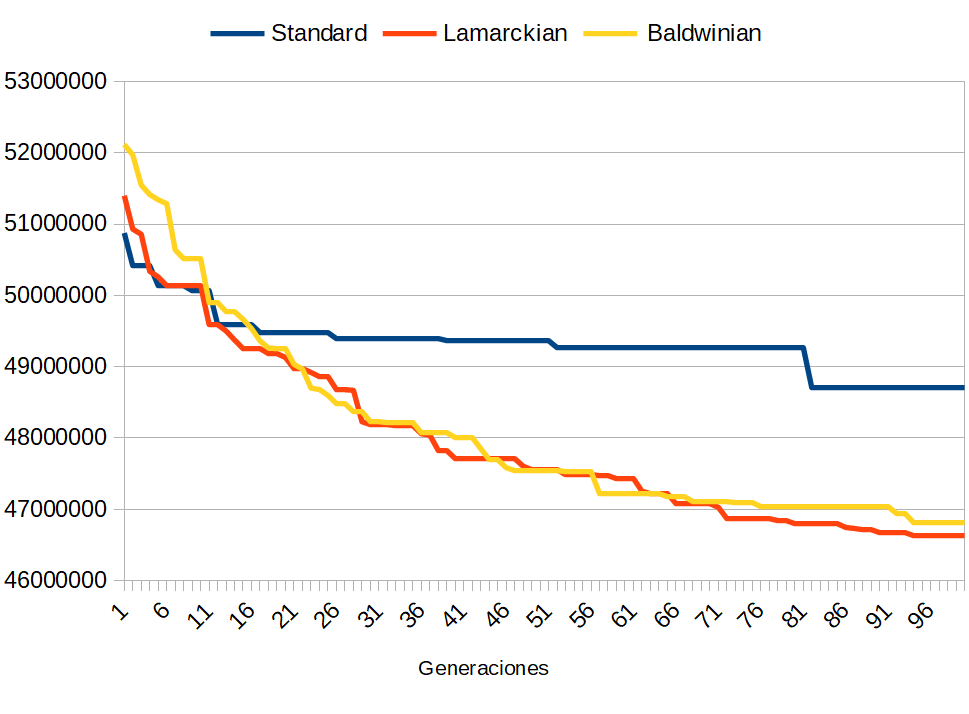
\includegraphics[width=1\textwidth]{../images/comparacion-3}
  \caption{Comparación del resultado de la ejecución de los tres algoritmos}
  \label{fig:comparacion-3}
\end{figure}

Se han repetido las ejecuciones varias veces con resultados muy parecidos, por lo que se concluye que estos datos son representativos.

Como puede verse, el algoritmo que peor desempeño tiene es el estándar, ya que mejora muy poco y muy lentamente a lo largo de su ejecución. Por otro lado, sus dos variantes tienen resultados bastante parecidos, aunque la implementación lamarckiana da mejores resultados. Esto tiene sentido, ya que transmitir las mejoras de un individuo en sus cromosomas, aunque no sea realista, proporciona mejores resultados que de no hacerlo.


\section{Mejor resultado obtenido}

Actualmente, el mejor resultado obtenido ha sido con la ejecución de la implementación \textbf{lamarckiana} con un fitness de \textbf{46634000}, un $\sim$1.06\% mayor que la cota inferior global conocida (44095032). Sus cromosomas pueden verse en el anexo \ref{anexo:best}.